\documentclass{article}
\usepackage[utf8]{inputenc}
\usepackage{graphicx}

% change reference style to [1], remove stupid sorting, language changed so date in ddmmyyyy
\usepackage[backend=biber, style=numeric, sorting=none, language=australian]{biblatex}
\addbibresource{References.bib}

\title{Report:\\
    \large Project Specification
}
\author{David Saunders (910995)}
\date{April 2020}

\begin{document}
\maketitle

\begin{abstract} 
    Write abstract here
\end{abstract}

\tableofcontents

\section{Mark scheme}
This coursework contributes 50\% of the mark for the module. The size is
approximately 5000 words (excluding references) – due on Wednesday 29
April 2020 (11:00 am).

This report should give a literature review over your project and describe
any background research that you have carried out. You should state the motivation and aims of the project. It should include a complete specification
of your project. It should describe the project clearly and the components
of the work which need to be developed. An outline project plan for the
summer should be included. This plan should take into account the development methodology being used. You should provide a risk analysis for the
project. You should view this document as providing the plan for the work
you expect to carry out over the summer.

\section{Literature review}

Write section 1 here \cite{torsney2011tuner} and talk about figure \ref{fig:test}.

This can pretty much be the review I did for the first assignment. 

\begin{figure}[ht]
    \centering
    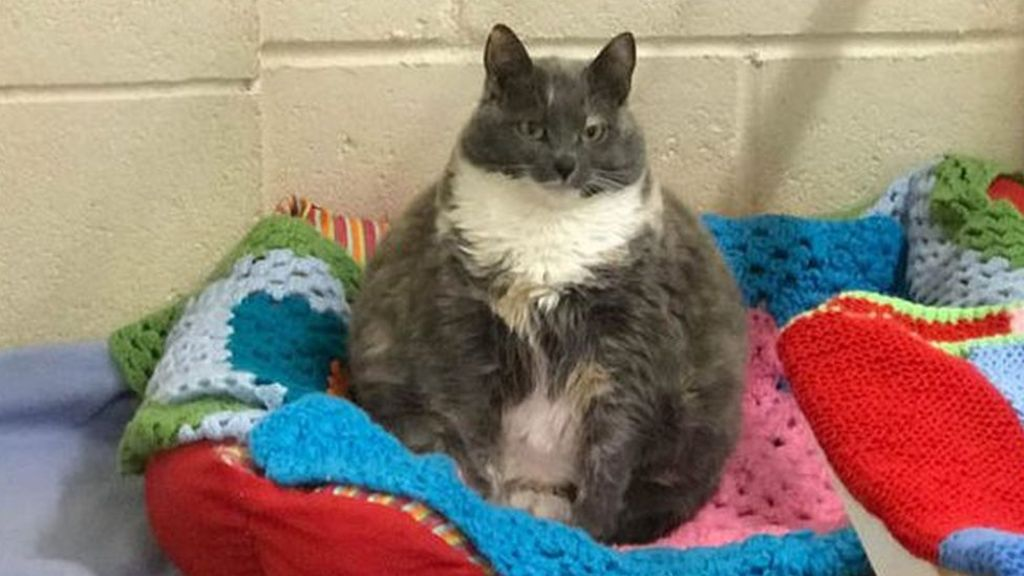
\includegraphics[scale=0.35]{Test.JPG}
    \caption{This will be a figure showcasing some of my work}
    \label{fig:test}
\end{figure}

\section{Background Research}
Anything I've looked at with help for mouse data classification algorithms? 


\section{Motivation and Aims of project}
Can copy from presentation slides but fill in so they're more wordy.


\section{Project plan}

\subsection{Development methodology}
Discuss software life cycle methodologies with Jacques.
An agile methodology such as scrum would probably be best but am I constrained  by this specification document?

\begin{figure}[ht]
    \centering
    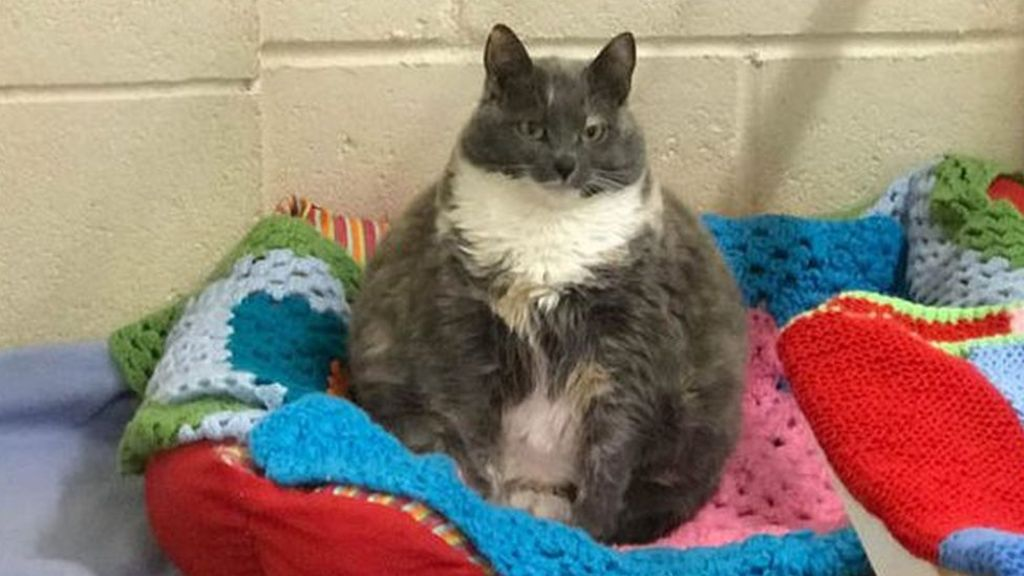
\includegraphics[scale=0.35]{Test.JPG}
    \caption{A Gantt chart showing the planned milestones of the project.}
    \label{fig:Gantt}
\end{figure}

\section{Risk Analysis}
Copy this from my project last year.

Risks: 
- BIGGEST we find that there is no correlation between attendtion and mouse data and nothing is prooved.
- COID19 effecting the UK more. - I was considering running more lab studies to get more data but the shutdown has stopped that ambishion.
    It has already effected, anything worse like close family and elderly parents getting ill so supervisor or me would be a risk.
    Plan ahead, wash hands.


\printbibliography

\end{document}